From the analysis of the results of the measurements in Appendix \autoref{App2}, it is shown, that the height of the antennas and the distance between them have a much higher influence on the PL, than the other parameters, which is the placement, antenna type and polarization. As these parameters have a much less influence on the PL, there will only be focused on the different height combinations and distance between the antennas.

Firstly there will be looked at the case, where the height of the transmitting antenna and the receiving antenna is at the same heights, over the different distance.

\begin{figure}[!htbp]
\centering
% This file was created by matlab2tikz.
%
%The latest updates can be retrieved from
%  http://www.mathworks.com/matlabcentral/fileexchange/22022-matlab2tikz-matlab2tikz
%where you can also make suggestions and rate matlab2tikz.
%
\definecolor{mycolor1}{rgb}{0.00000,0.44700,0.74100}%
\definecolor{mycolor2}{rgb}{0.85000,0.32500,0.09800}%
\definecolor{mycolor3}{rgb}{0.92900,0.69400,0.12500}%
\definecolor{mycolor4}{rgb}{0.49400,0.18400,0.55600}%
%
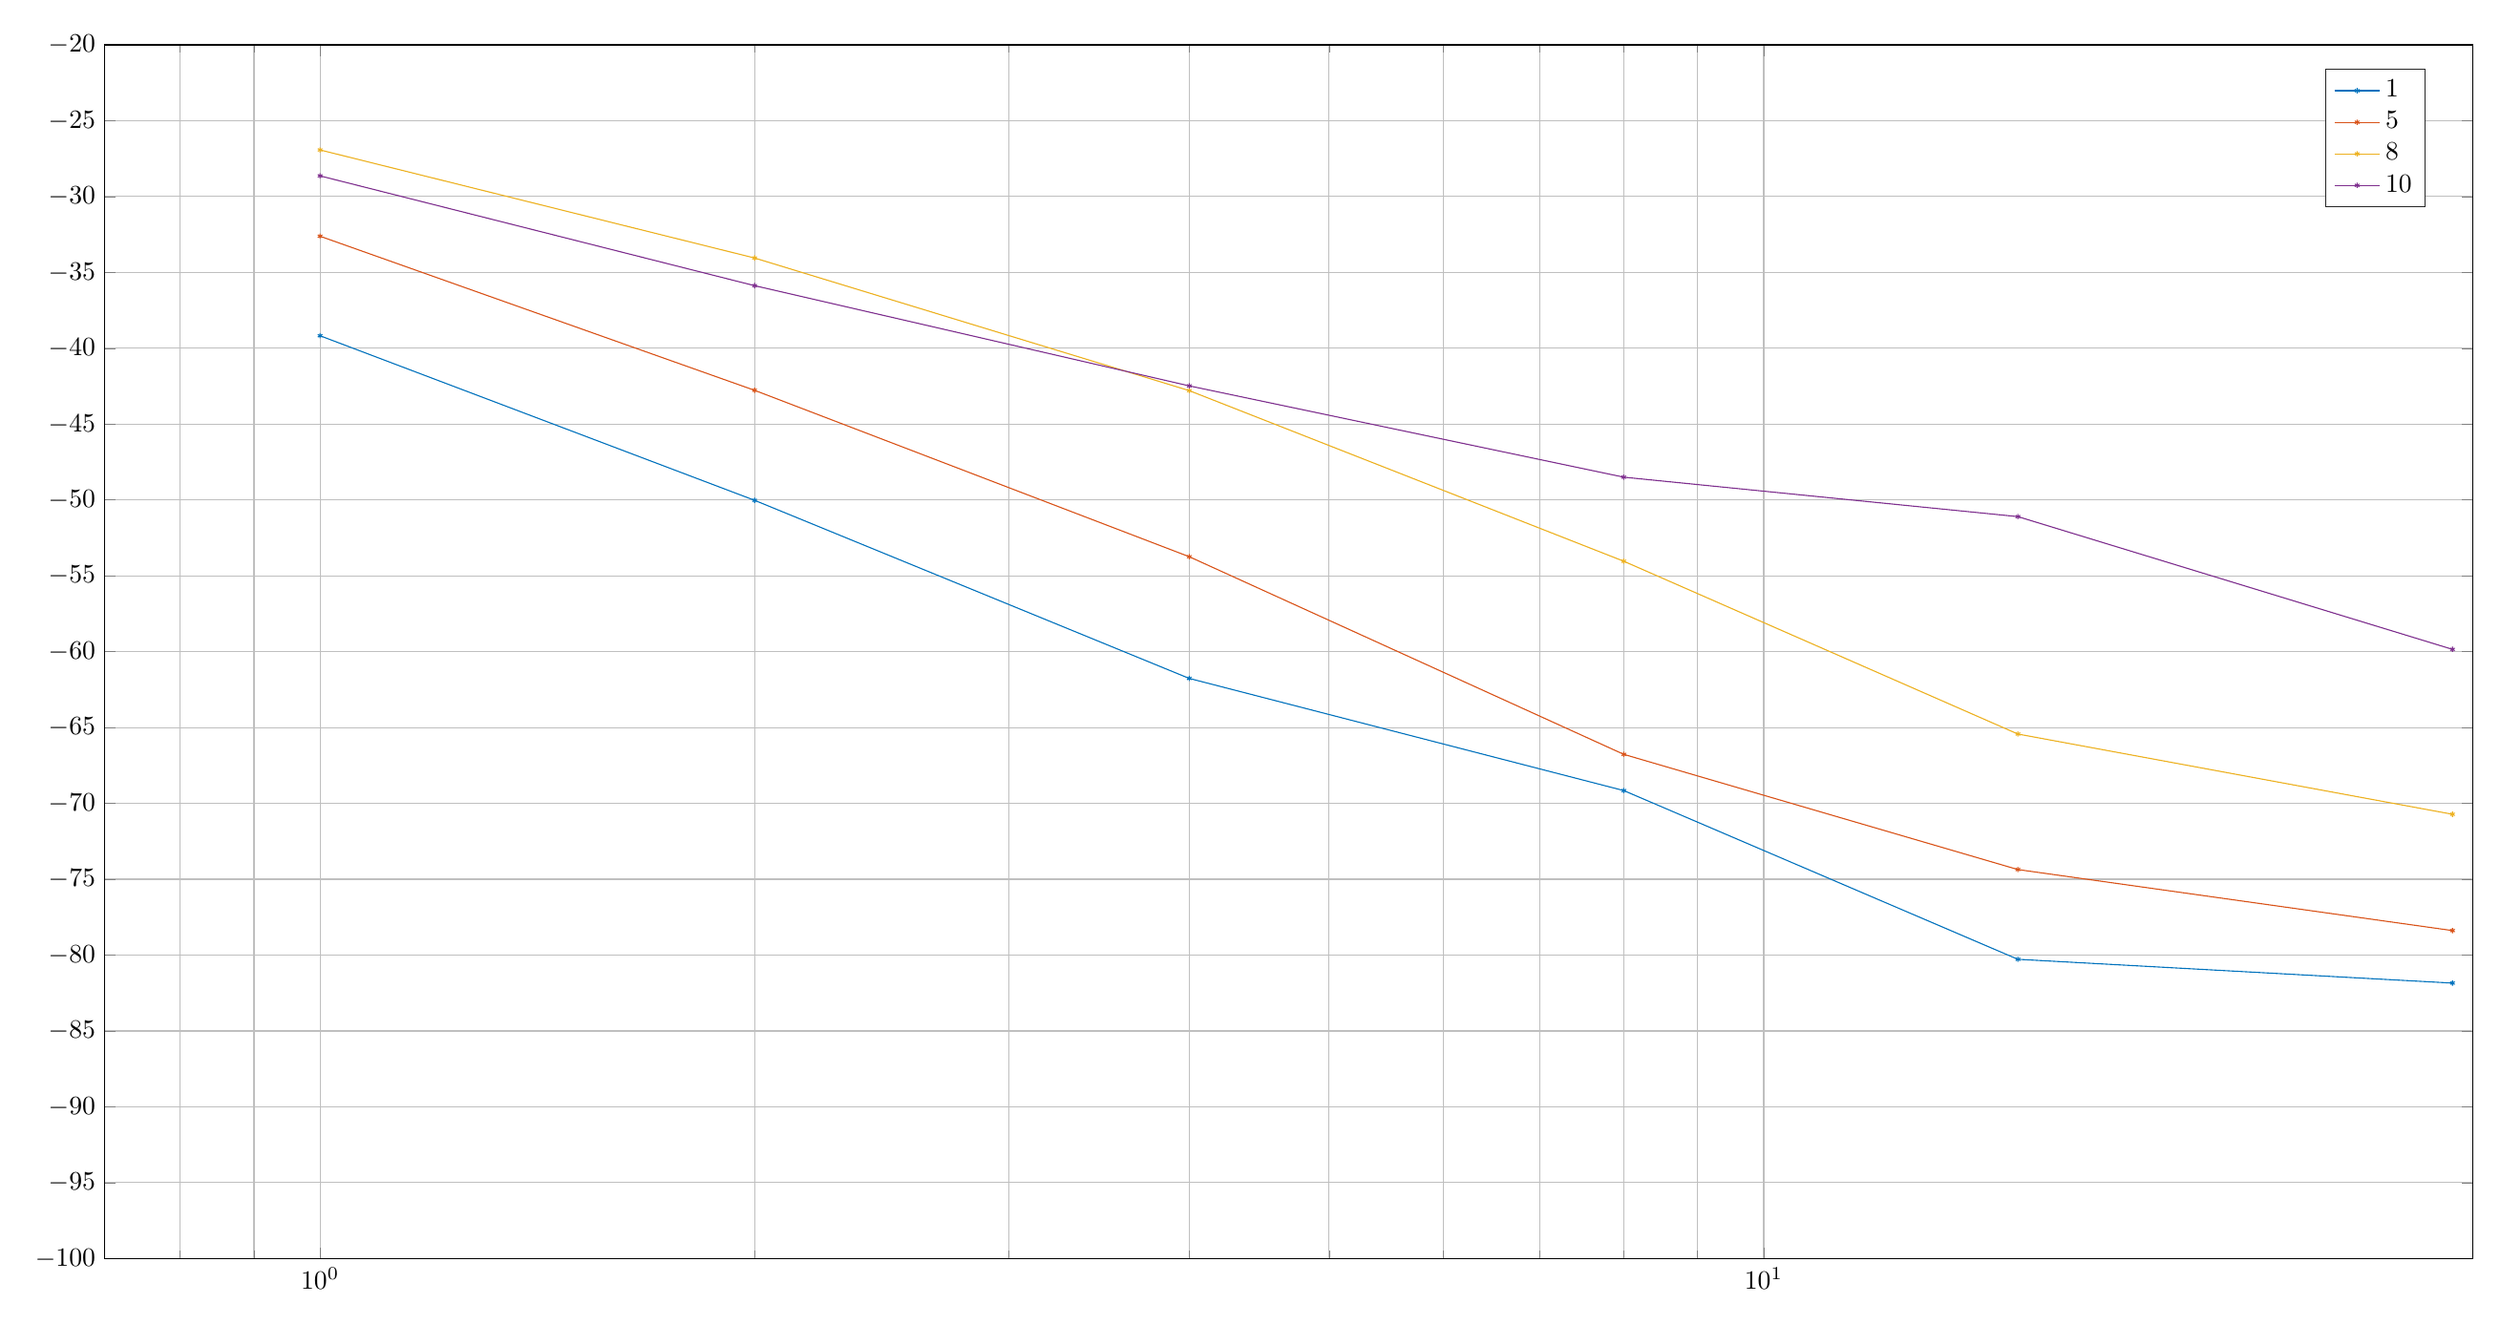
\begin{tikzpicture}

\begin{axis}[%
width=12.4in,
height=6.357in,
at={(2.08in,0.858in)},
scale only axis,
xmode=log,
xmin=0,
xmax=31,
xminorticks=true,
xmajorgrids,
xminorgrids,
ymin=-100,
ymax=-20,
ymajorgrids,
axis background/.style={fill=white},
legend style={legend cell align=left,align=left,draw=white!15!black}
]
\addplot [color=mycolor1,solid,mark size=1.0pt,mark=asterisk,mark options={solid}]
  table[row sep=crcr]{%
1	-39.176832441447\\
2	-50.0236813268286\\
4	-61.7627349006033\\
8	-69.1568155321866\\
15	-80.2784721484843\\
30	-81.8463231335614\\
};
\addlegendentry{1};

\addplot [color=mycolor2,solid,mark size=1.0pt,mark=asterisk,mark options={solid}]
  table[row sep=crcr]{%
1	-32.6162301822822\\
2	-42.7733202106742\\
4	-53.7406598744587\\
8	-66.7692891298477\\
15	-74.3619892107941\\
30	-78.384604174472\\
};
\addlegendentry{5};

\addplot [color=mycolor3,solid,mark size=1.0pt,mark=asterisk,mark options={solid}]
  table[row sep=crcr]{%
1	-26.9292301822822\\
2	-34.0517673842044\\
4	-42.7927848744587\\
8	-54.0404141298477\\
15	-65.4297392107941\\
30	-70.718229174472\\
};
\addlegendentry{8};

\addplot [color=mycolor4,solid,mark size=1.0pt,mark=asterisk,mark options={solid}]
  table[row sep=crcr]{%
1	-28.6391813268286\\
2	-35.8754849006033\\
4	-42.4804405321866\\
8	-48.4989721484843\\
15	-51.0989481335614\\
30	-59.847479174472\\
};
\addlegendentry{10};

\end{axis}
\end{tikzpicture}%
\caption{Mesurements of PL for transmitter and receiver antenna at the same height, at varying distance.}
\label{Meas1}
\end{figure}

It is seen on \autoref{Meas1}, that the longer the distance, the higher the PL. This comes from the same principle, that the FSPL model is based on, which is given as signal = $\frac{1}{d^{2}}$, this means that the larger the distance the less signal is obtained, and more PL loss. When looking at the graph compared to changing the heights, it is seen, that the lower the antennas is placed, the higher PL. This comes from the principle, that reflections comes from the ground and comes with (in most cases) destructive interference, which the TRPL model is based on. 

Secondly there will be looked at the case, where the height of the transmitting antenna is kept at a single height, both low at 0.01m \autoref{Meas2} and high at 2.00m \autoref{Meas3}, while the height of the receiving antenna is varying.

\begin{figure}[!htbp]
\centering
% This file was created by matlab2tikz.
%
%The latest updates can be retrieved from
%  http://www.mathworks.com/matlabcentral/fileexchange/22022-matlab2tikz-matlab2tikz
%where you can also make suggestions and rate matlab2tikz.
%
\definecolor{mycolor1}{rgb}{0.00000,0.44700,0.74100}%
\definecolor{mycolor2}{rgb}{0.85000,0.32500,0.09800}%
\definecolor{mycolor3}{rgb}{0.92900,0.69400,0.12500}%
\definecolor{mycolor4}{rgb}{0.49400,0.18400,0.55600}%
%
\begin{tikzpicture}

\begin{axis}[%
width=2.8in,
height=\myvar,
at={(2.08in,0.858in)},
scale only axis,
xmode=log,
xmin=0.9,
xmax=31,
xlabel=Distance (m),
xminorticks=true,
xmajorgrids,
xminorgrids,
ymin=20,
ymax=100,
ylabel=Path loss (dB),
ymajorgrids,
legend pos = north west,
axis background/.style={fill=white},
legend style={legend cell align=left,align=left,draw=white!15!black}
]
\addplot [color=mycolor1,solid,mark size=1.0pt,mark=asterisk,mark options={solid}]
  table[row sep=crcr]{%
1	39.176832441447\\
2	50.0236813268286\\
4	61.7627349006033\\
8	69.1568155321866\\
15	80.2784721484843\\
30	81.8463231335614\\
};
\addlegendentry{0.04m};

\addplot [color=mycolor2,solid,mark size=1.0pt,mark=asterisk,mark options={solid}]
  table[row sep=crcr]{%
1.00422308278589	36.2750685665333\\
2.00211488181872	46.4255855564945\\
4.0010578601165	56.521087110148\\
8.00052898251109	65.8421427417313\\
15.0002821306801	78.7553243580291\\
30.000141066335	80.3591753431061\\
};
\addlegendentry{0.14m};

\addplot [color=mycolor3,solid,mark size=1.0pt,mark=asterisk,mark options={solid}]
  table[row sep=crcr]{%
1.05621967412087	33.1826999363486\\
2.02869416127715	41.0212571697177\\
4.01442399355125	51.2789435665333\\
8.0072217404041	62.2242106975379\\
15.0038528385212	70.1578243580291\\
30.0019266048032	74.3636753431061\\
};
\addlegendentry{0.36m};

\addplot [color=mycolor4,solid,mark size=1.0pt,mark=asterisk,mark options={solid}]
  table[row sep=crcr]{%
2.23606797749979	40.2024392944793\\
2.82842712474619	41.1498149750094\\
4.47213595499958	45.3166779228563\\
8.24621125123532	51.29571423555\\
15.1327459504216	61.8265071697177\\
30.0665927567458	73.152023643832\\
};
\addlegendentry{2.02m};

\end{axis}
\end{tikzpicture}%
\caption{Mesurements of PL for transmitter at 0.01m and receiver antenna at varying heights}
\label{Meas2}
\end{figure}

\begin{figure}[!htbp]
\centering
% This file was created by matlab2tikz.
%
%The latest updates can be retrieved from
%  http://www.mathworks.com/matlabcentral/fileexchange/22022-matlab2tikz-matlab2tikz
%where you can also make suggestions and rate matlab2tikz.
%
\definecolor{mycolor1}{rgb}{0.00000,0.44700,0.74100}%
\definecolor{mycolor2}{rgb}{0.85000,0.32500,0.09800}%
\definecolor{mycolor3}{rgb}{0.92900,0.69400,0.12500}%
\definecolor{mycolor4}{rgb}{0.49400,0.18400,0.55600}%
%
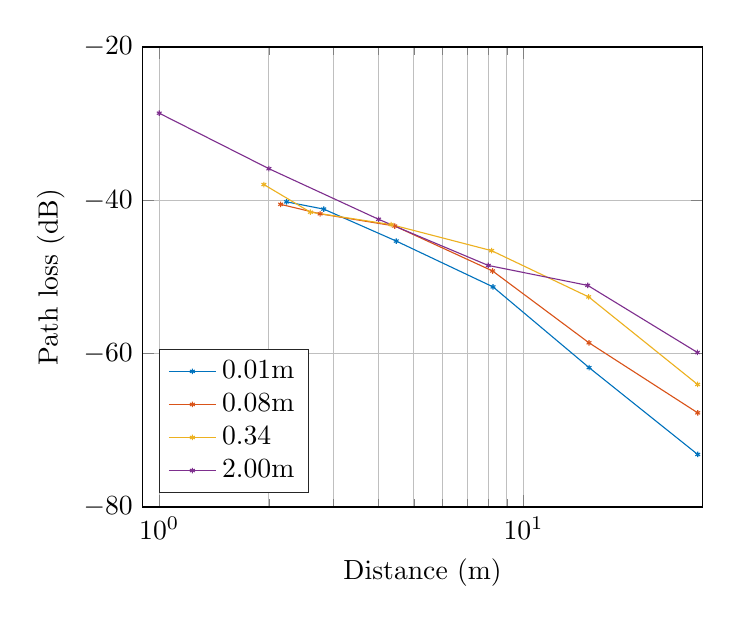
\begin{tikzpicture}

\begin{axis}[%
width=2.8in,
height=2.3in,
at={(2.08in,0.858in)},
scale only axis,
xmode=log,
xmin=0.9,
xmax=31,
xlabel=Distance (m),
xminorticks=true,
xmajorgrids,
xminorgrids,
ymin=-80,
ymax=-20,
ylabel=Path loss (dB),
ymajorgrids,
legend pos = south west,
axis background/.style={fill=white},
legend style={legend cell align=left,align=left,draw=white!15!black}
]
\addplot [color=mycolor1,solid,mark size=1.0pt,mark=asterisk,mark options={solid}]
  table[row sep=crcr]{%
2.23606797749979	-40.2024392944793\\
2.82842712474619	-41.1498149750094\\
4.47213595499958	-45.3166779228563\\
8.24621125123532	-51.29571423555\\
15.1327459504216	-61.8265071697177\\
30.0665927567458	-73.152023643832\\
};
\addlegendentry{0.01m};

\addplot [color=mycolor2,solid,mark size=1.0pt,mark=asterisk,mark options={solid}]
  table[row sep=crcr]{%
2.1541736234575	-40.5286184873639\\
2.7641389255969	-41.7634386176021\\
4.43175631099003	-43.3569736894665\\
8.22438228683468	-49.22358923555\\
15.1208618801972	-58.5868821697177\\
30.060613167399	-67.725648643832\\
};
\addlegendentry{0.08m};

\addplot [color=mycolor3,solid,mark size=1.0pt,mark=asterisk,mark options={solid}]
  table[row sep=crcr]{%
1.93793704748116	-37.947787309918\\
2.59915370842126	-41.5490546940608\\
4.33077360294902	-43.1688945864033\\
8.17041002643074	-46.5688884715957\\
15.0915738079234	-52.6026681377669\\
30.0458915660694	-64.022898643832\\
};
\addlegendentry{0.34};

\addplot [color=mycolor4,solid,mark size=1.0pt,mark=asterisk,mark options={solid}]
  table[row sep=crcr]{%
1	-28.6391813268286\\
2	-35.8754849006033\\
4	-42.4804405321866\\
8	-48.4989721484843\\
15	-51.0989481335614\\
30	-59.847479174472\\
};
\addlegendentry{2.00m};

\end{axis}
\end{tikzpicture}%
\caption{Mesurements of PL for transmitter at 2.00m and receiver antenna at varying heights}
\label{Meas3}
\end{figure}

In both cases, it is seen that the lower the heights of the antennas is, the higher the PL. Some of the measurements are very close at the short distance on \autoref{Meas3}. This comes from the destructive interference, that comes at different angles. As the different heights of the receiver antenna gives different angles, where the difference is much higher close by the transmitter antenna, the difference in destructive interference is larger and the measurements get closer to each other.

Lastly there will make a comparison of the measured data and the model described earlier, to see if the model estimated the measured data correctly, this is done at at selected Tx and Rx as seen on \autoref{Models1}, \autoref{Models7} and \autoref{Models10}.

%THOMAS, INSERT FIGURER HER, SOM VISER AT DE FORSKELLIGE MODELLER VIRKER I FORSKELLIGE OMRÅDE... SÅ BURDE DU HAVE EN GOD NOK OVERGANG TIL DIT :)


\begin{figure}[!htbp]
\centering
\input{figures/Models1.tex}
\caption{Comparison between measured path loss and predicted path loss from models at a Tx and Rx height of 0.04 m}
\label{Models1}
\end{figure}

On \autoref{Models1} it can be seen that GWPL and NSPL predicts the PL best, however both model overestimate the PL by close to 10 dB, which could indicate that the measurements of $\epsilon_0$ might not be completely accurate. Here the general problem with low heigth is also seen as FSPL greatly underestimate the PL where TRPL greatly overestimate the PL.

\begin{figure}[!htbp]
\centering
% This file was created by matlab2tikz.
%
%The latest updates can be retrieved from
%  http://www.mathworks.com/matlabcentral/fileexchange/22022-matlab2tikz-matlab2tikz
%where you can also make suggestions and rate matlab2tikz.
%
\definecolor{mycolor1}{rgb}{0.00000,0.44700,0.74100}%
\definecolor{mycolor2}{rgb}{0.85000,0.32500,0.09800}%
\definecolor{mycolor3}{rgb}{0.92900,0.69400,0.12500}%
\definecolor{mycolor4}{rgb}{0.49400,0.18400,0.55600}%
\definecolor{mycolor5}{rgb}{0.46600,0.67400,0.18800}%
%
\begin{tikzpicture}

\begin{axis}[%
width=2.8in,
height=\myvar,
at={(0.758in,0.481in)},
scale only axis,
xmode=log,
extra x ticks={2,5,20}, 
extra x tick style={log identify minor tick positions=false},
log ticks with fixed point,
xmin=0.9,
xmax=31,
xlabel=Distance (m),
xminorticks=true,
xmajorgrids,
xminorgrids,
ymin=20,
ymax=100,
ylabel=Path loss (dB),
ymajorgrids,
axis background/.style={fill=white},
legend style={legend cell align=left,align=left,draw=white!15!black},
legend pos = north west
]
\addplot [color=mycolor1,mark size=2.5pt,only marks,mark=asterisk,mark options={solid}]
  table[row sep=crcr]{%
2.1541736234575	40.5286184873639\\
2.7641389255969	41.7634386176021\\
4.43175631099003	43.3569736894665\\
8.22438228683468	49.22358923555\\
15.1208618801972	58.5868821697177\\
30.060613167399	67.725648643832\\
};
\addlegendentry{Measured PL};
\addplot [color=mycolor2,solid]
  table[row sep=crcr]{%
1	31.1115179430228\\
1.29292929292929	33.3430134440292\\
1.58585858585859	35.1168070992565\\
1.87878787878788	36.5890729354301\\
2.17171717171717	37.8475832493839\\
2.46464646464646	38.9466105778464\\
2.75757575757576	39.9220669918869\\
3.05050505050505	40.7989529102148\\
3.34343434343434	41.5953739265862\\
3.63636363636364	42.3248640664175\\
3.92929292929293	42.9978060775859\\
4.22222222222222	43.6223396865725\\
4.51515151515152	44.2049645137105\\
4.80808080808081	44.7509531054816\\
5.1010101010101	45.264641613445\\
5.39393939393939	45.7496391916429\\
5.68686868686869	46.2089819480987\\
5.97979797979798	46.6452481855302\\
6.27272727272727	47.0606460546034\\
6.56565656565657	47.4570811839289\\
6.85858585858586	47.8362095366818\\
7.15151515151515	48.1994792048672\\
7.44444444444444	48.5481638082528\\
7.73737373737374	48.8833894437239\\
8.03030303030303	49.2061566242012\\
8.32323232323232	49.5173582850141\\
8.61616161616162	49.8177946744222\\
8.90909090909091	50.1081857537082\\
9.2020202020202	50.3891815905317\\
9.49494949494949	50.6613711230658\\
9.78787878787879	50.9252895920871\\
10.0808080808081	51.1814248768192\\
};
\addlegendentry{FSPL};
\addplot [color=mycolor2,dashed,forget plot]
  table[row sep=crcr]{%
3.34343434343434	41.5953739265862\\
3.63636363636364	42.3248640664175\\
3.92929292929293	42.9978060775859\\
4.22222222222222	43.6223396865725\\
4.51515151515152	44.2049645137105\\
4.80808080808081	44.7509531054816\\
5.1010101010101	45.264641613445\\
5.39393939393939	45.7496391916429\\
5.68686868686869	46.2089819480987\\
5.97979797979798	46.6452481855302\\
6.27272727272727	47.0606460546034\\
6.56565656565657	47.4570811839289\\
6.85858585858586	47.8362095366818\\
7.15151515151515	48.1994792048672\\
7.44444444444444	48.5481638082528\\
7.73737373737374	48.8833894437239\\
8.03030303030303	49.2061566242012\\
8.32323232323232	49.5173582850141\\
8.61616161616162	49.8177946744222\\
8.90909090909091	50.1081857537082\\
9.2020202020202	50.3891815905317\\
9.49494949494949	50.6613711230658\\
9.78787878787879	50.9252895920871\\
10.0808080808081	51.1814248768192\\
10.3737373737374	51.4302229230174\\
10.6666666666667	51.6720924150277\\
10.959595959596	51.9074088147627\\
11.2525252525253	52.136517867826\\
11.5454545454545	52.3597386589774\\
11.8383838383838	52.5773662847132\\
12.1313131313131	52.7896741991299\\
12.4242424242424	52.9969162798597\\
12.7171717171717	53.199328653229\\
13.010101010101	53.3971313115477\\
13.3030303030303	53.5905295503075\\
13.5959595959596	53.7797152488309\\
13.8888888888889	53.9648680143974\\
14.1818181818182	54.1461562069475\\
14.4747474747475	54.3237378590187\\
14.7676767676768	54.4977615035086\\
15.0606060606061	54.6683669201317\\
15.3535353535354	54.8356858099672\\
15.6464646464646	54.9998424062559\\
15.9393939393939	55.1609540285398\\
16.2323232323232	55.3191315863387\\
16.5252525252525	55.4744800377779\\
16.8181818181818	55.6270988079186\\
17.1111111111111	55.7770821709656\\
17.4040404040404	55.9245196000324\\
17.6969696969697	56.069496087713\\
17.989898989899	56.2120924403367\\
18.2828282828283	56.3523855484555\\
18.5757575757576	56.4904486358333\\
18.8686868686869	56.6263514889533\\
19.1616161616162	56.760160668845\\
19.4545454545455	56.8919397068421\\
19.7474747474747	57.0217492857095\\
20.040404040404	57.149647407435\\
20.3333333333333	57.2756895488449\\
20.6262626262626	57.3999288060896\\
20.9191919191919	57.5224160289408\\
21.2121212121212	57.6431999457502\\
21.5050505050505	57.7623272798382\\
21.7979797979798	57.8798428580096\\
22.0909090909091	57.9957897118245\\
22.3838383838384	58.1102091721996\\
22.6767676767677	58.2231409578586\\
22.969696969697	58.3346232581061\\
23.2626262626263	58.4446928103564\\
23.5555555555556	58.5533849728113\\
23.8484848484848	58.6607337926463\\
24.1414141414141	58.7667720700345\\
24.4343434343434	58.8715314183094\\
24.7272727272727	58.9750423205423\\
25.020202020202	59.0773341827885\\
25.3131313131313	59.1784353842344\\
25.6060606060606	59.2783733244589\\
25.8989898989899	59.3771744680074\\
26.1919191919192	59.4748643864588\\
26.4848484848485	59.5714677981531\\
26.7777777777778	59.6670086057337\\
27.0707070707071	59.7615099316476\\
27.3636363636364	59.8549941517351\\
27.6565656565657	59.9474829270312\\
27.9494949494949	60.0389972338908\\
28.2424242424242	60.1295573925447\\
28.5353535353535	60.2191830941809\\
28.8282828282828	60.3078934266443\\
29.1212121212121	60.3957068988359\\
29.4141414141414	60.4826414638918\\
29.7070707070707	60.5687145412132\\
30	60.653943037416\\
};

\addplot [color=mycolor3,dashed,forget plot]
  table[row sep=crcr]{%
1	11.1879572974509\\
1.29292929292929	15.6509482994637\\
1.58585858585859	19.1985356099183\\
1.87878787878788	22.1430672822656\\
2.17171717171717	24.6600879101731\\
2.46464646464646	26.8581425670981\\
2.75757575757576	28.8090553951792\\
3.05050505050505	30.562827231835\\
3.34343434343434	32.1556692645777\\
3.63636363636364	33.6146495442404\\
3.92929292929293	34.9605335665772\\
4.22222222222222	36.2096007845503\\
4.51515151515152	37.3748504388264\\
4.80808080808081	38.4668276223687\\
5.1010101010101	39.4942046382954\\
5.39393939393939	40.4641997946912\\
5.68686868686869	41.3828853076028\\
5.97979797979798	42.2554177824657\\
6.27272727272727	43.0862135206121\\
6.56565656565657	43.8790837792632\\
6.85858585858586	44.637340484769\\
7.15151515151515	45.3638798211397\\
7.44444444444444	46.061249027911\\
7.73737373737374	46.7317002988531\\
8.03030303030303	47.3772346598077\\
8.32323232323232	47.9996379814336\\
8.61616161616162	48.6005107602498\\
8.90909090909091	49.1812929188217\\
9.2020202020202	49.7432845924689\\
9.49494949494949	50.2876636575369\\
9.78787878787879	50.8155005955795\\
10.0808080808081	51.3277711650438\\
10.3737373737374	51.8253672574401\\
10.6666666666667	52.3091062414607\\
10.959595959596	52.7797390409309\\
11.2525252525253	53.2379571470573\\
};

\addplot [color=mycolor3,solid]
  table[row sep=crcr]{%
10.0808080808081	51.3277711650438\\
10.3737373737374	51.8253672574401\\
10.6666666666667	52.3091062414607\\
10.959595959596	52.7797390409309\\
11.2525252525253	53.2379571470573\\
11.5454545454545	53.6843987293602\\
11.8383838383838	54.1196539808318\\
12.1313131313131	54.5442698096652\\
12.4242424242424	54.9587539711248\\
12.7171717171717	55.3635787178634\\
13.010101010101	55.7591840345007\\
13.3030303030303	56.1459805120203\\
13.5959595959596	56.5243519090673\\
13.8888888888889	56.8946574402002\\
14.1818181818182	57.2572338253004\\
14.4747474747475	57.6123971294427\\
14.7676767676768	57.9604444184226\\
15.0606060606061	58.3016552516687\\
15.3535353535354	58.6362930313398\\
15.6464646464646	58.9646062239172\\
15.9393939393939	59.286829468485\\
16.2323232323232	59.6031845840827\\
16.5252525252525	59.9138814869611\\
16.8181818181818	60.2191190272425\\
17.1111111111111	60.5190857533365\\
17.4040404040404	60.8139606114701\\
17.6969696969697	61.1039135868314\\
17.989898989899	61.3891062920787\\
18.2828282828283	61.6696925083163\\
18.5757575757576	61.945818683072\\
18.8686868686869	62.2176243893119\\
19.1616161616162	62.4852427490954\\
19.4545454545455	62.7488008250896\\
19.7474747474747	63.0084199828244\\
20.040404040404	63.2642162262753\\
20.3333333333333	63.5163005090951\\
20.6262626262626	63.7647790235846\\
20.9191919191919	64.009753469287\\
21.2121212121212	64.2513213029057\\
21.5050505050505	64.4895759710818\\
21.7979797979798	64.7246071274246\\
22.0909090909091	64.9565008350544\\
22.3838383838384	65.1853397558046\\
22.6767676767677	65.4112033271226\\
22.969696969697	65.6341679276176\\
23.2626262626263	65.8543070321182\\
23.5555555555556	66.071691357028\\
23.8484848484848	66.286388996698\\
24.1414141414141	66.4984655514744\\
24.4343434343434	66.7079842480241\\
24.7272727272727	66.9150060524899\\
25.020202020202	67.1195897769824\\
25.3131313131313	67.3217921798742\\
25.6060606060606	67.5216680603231\\
25.8989898989899	67.7192703474201\\
26.1919191919192	67.914650184323\\
26.4848484848485	68.1078570077116\\
26.7777777777778	68.2989386228727\\
27.0707070707071	68.4879412747005\\
27.3636363636364	68.6749097148757\\
27.6565656565657	68.8598872654678\\
27.9494949494949	69.042915879187\\
28.2424242424242	69.2240361964947\\
28.5353535353535	69.4032875997672\\
28.8282828282828	69.5807082646941\\
29.1212121212121	69.7563352090772\\
29.4141414141414	69.9302043391889\\
29.7070707070707	70.1023504938317\\
30	70.2728074862374\\
};
\addlegendentry{ATRPL};

\addplot [color=mycolor4,solid]
  table[row sep=crcr]{%
1	30.7915254982822\\
1.29292929292929	33.9434222862678\\
1.58585858585859	35.5316616445846\\
1.87878787878788	36.4283000798175\\
2.17171717171717	37.1924057499839\\
2.46464646464646	37.8719108333566\\
2.75757575757576	38.5554435638167\\
3.05050505050505	39.2675570359689\\
3.34343434343434	40.0024398250219\\
3.63636363636364	40.7481405071393\\
3.92929292929293	41.4941128854543\\
4.22222222222222	42.2326695378301\\
4.51515151515152	42.95868364737\\
4.80808080808081	43.6689535858759\\
5.1010101010101	44.3616304081836\\
5.39393939393939	45.0357852429981\\
5.68686868686869	45.6911029557652\\
5.97979797979798	46.3276711042173\\
6.27272727272727	46.945836254252\\
6.56565656565657	47.5461066501664\\
6.85858585858586	48.1290864581166\\
7.15151515151515	48.6954314624322\\
7.44444444444444	49.2458193563392\\
7.73737373737374	49.7809299882535\\
8.03030303030303	50.3014324189399\\
8.32323232323232	50.8079766484679\\
8.61616161616162	51.3011885476373\\
8.90909090909091	51.7816669857065\\
9.2020202020202	52.2499824573702\\
9.49494949494949	52.7066767250179\\
9.78787878787879	53.152263139189\\
10.0808080808081	53.5872274020081\\
10.3737373737374	54.0120286094323\\
10.6666666666667	54.4271004579408\\
10.959595959596	54.8328525363514\\
11.2525252525253	55.2296716481953\\
11.5454545454545	55.6179231276041\\
11.8383838383838	55.9979521240634\\
12.1313131313131	56.3700848401753\\
12.4242424242424	56.7346297127695\\
12.7171717171717	57.0918785320623\\
13.010101010101	57.4421074965988\\
13.3030303030303	57.7855782038035\\
13.5959595959596	58.1225385773774\\
13.8888888888889	58.4532237337049\\
14.1818181818182	58.7778567900119\\
14.4747474747475	59.0966496173513\\
14.7676767676768	59.4098035416476\\
15.0606060606061	59.7175099960736\\
15.3535353535354	60.0199511279849\\
15.6464646464646	60.317300363539\\
15.9393939393939	60.6097229329916\\
16.2323232323232	60.8973763595041\\
16.5252525252525	61.1804109141314\\
16.8181818181818	61.4589700394879\\
17.1111111111111	61.7331907444194\\
17.4040404040404	62.0032039718441\\
17.6969696969697	62.2691349417683\\
17.989898989899	62.5311034713306\\
18.2828282828283	62.7892242735887\\
18.5757575757576	63.0436072366292\\
18.8686868686869	63.2943576844593\\
19.1616161616162	63.5415766210216\\
19.4545454545455	63.7853609585727\\
19.7474747474747	64.025803731563\\
20.040404040404	64.2629942970691\\
20.3333333333333	64.4970185227456\\
20.6262626262626	64.727958963188\\
20.9191919191919	64.9558950255269\\
21.2121212121212	65.1809031250124\\
21.5050505050505	65.4030568312845\\
21.7979797979798	65.622427005976\\
22.0909090909091	65.8390819322413\\
22.3838383838384	66.0530874367596\\
22.6767676767677	66.2645070047219\\
22.969696969697	66.4734018882686\\
23.2626262626263	66.679831208813\\
23.5555555555556	66.8838520536515\\
23.8484848484848	67.0855195672332\\
24.1414141414141	67.2848870374317\\
24.4343434343434	67.4820059771411\\
24.7272727272727	67.6769262014908\\
25.020202020202	67.8696959009536\\
25.3131313131313	68.0603617106055\\
25.6060606060606	68.2489687757714\\
25.8989898989899	68.4355608142797\\
26.1919191919192	68.620180175531\\
26.4848484848485	68.8028678965711\\
26.7777777777778	68.9836637553483\\
27.0707070707071	69.1626063213201\\
27.3636363636364	69.3397330035641\\
27.6565656565657	69.5150800965393\\
27.9494949494949	69.688682823631\\
28.2424242424242	69.8605753786071\\
28.5353535353535	70.0307909651024\\
28.8282828282828	70.1993618342431\\
29.1212121212121	70.366319320513\\
29.4141414141414	70.5316938759595\\
29.7070707070707	70.6955151028293\\
30	70.8578117847193\\
};
\addlegendentry{GWPL};

\addplot [color=mycolor5,dashed,forget plot]
  table[row sep=crcr]{%
1	49.3538609508286\\
1.29292929292929	53.3959745464176\\
1.58585858585859	56.5207156914694\\
1.87878787878788	59.0676402548208\\
2.17171717171717	61.2264933448044\\
2.46464646464646	63.1104587867558\\
2.75757575757576	64.7902302190781\\
3.05050505050505	66.311830849943\\
3.34343434343434	67.7064887792703\\
3.63636363636364	68.996278663249\\
3.92929292929293	70.1974189696354\\
4.22222222222222	71.3222456849008\\
4.51515151515152	72.3804266076039\\
4.80808080808081	73.3797314926537\\
5.1010101010101	74.3265363364305\\
5.39393939393939	75.2261642665338\\
5.68686868686869	76.0831231335442\\
5.97979797979798	76.9012758912276\\
6.27272727272727	77.6839659897684\\
6.56565656565657	78.4341118308212\\
6.85858585858586	79.1542793983295\\
7.15151515151515	79.8467391285975\\
7.44444444444444	80.5135111519851\\
7.73737373737374	81.1564017871898\\
8.03030303030303	81.7770333396581\\
8.32323232323232	82.3768686939538\\
8.61616161616162	82.9572318016748\\
8.90909090909091	83.5193248929627\\
9.2020202020202	84.0642430434446\\
9.49494949494949	84.5929865853301\\
9.78787878787879	85.1064717453882\\
10.0808080808081	85.6055398128794\\
10.3737373737374	86.0909650798918\\
10.6666666666667	86.5634617498139\\
10.959595959596	87.0236899732883\\
11.2525252525253	87.4722611423495\\
11.5454545454545	87.9097425507082\\
11.8383838383838	88.3366615099201\\
12.1313131313131	88.7535089964717\\
12.4242424242424	89.1607428928525\\
12.7171717171717	89.5587908758959\\
13.010101010101	89.9480529976065\\
13.3030303030303	90.3289039970187\\
13.5959595959596	90.7016953760679\\
13.8888888888889	91.0667572678091\\
14.1818181818182	91.4244001214087\\
14.4747474747475	91.7749162250337\\
14.7676767676768	92.1185810849709\\
15.0606060606061	92.4556546769273\\
15.3535353535354	92.7863825834364\\
15.6464646464646	93.1109970295529\\
15.9393939393939	93.4297178275263\\
16.2323232323232	93.7427532398573\\
16.5252525252525	94.0503007690251\\
16.8181818181818	94.3525478812105\\
17.1111111111111	94.6496726705026\\
17.4040404040404	94.9418444693439\\
17.6969696969697	95.2292244103331\\
17.989898989899	95.5119659439452\\
18.2828282828283	95.7902153162385\\
18.5757575757576	96.0641120101891\\
18.8686868686869	96.3337891539123\\
19.1616161616162	96.5993738986962\\
19.4545454545455	96.8609877694759\\
19.7474747474747	97.1187469901163\\
20.040404040404	97.3727627856349\\
20.3333333333333	97.6231416632925\\
20.6262626262626	97.8699856742928\\
20.9191919191919	98.1133926576673\\
21.2121212121212	98.3534564677773\\
21.5050505050505	98.5902671867284\\
21.7979797979798	98.8239113228803\\
22.0909090909091	99.0544719965241\\
22.3838383838384	99.2820291137069\\
22.6767676767677	99.5066595290969\\
22.969696969697	99.7284371987036\\
23.2626262626263	99.9474333232019\\
23.5555555555556	100.163716482539\\
23.8484848484848	100.377352762456\\
24.1414141414141	100.588405873489\\
24.4343434343434	100.796937262992\\
24.7272727272727	101.003006220645\\
25.020202020202	101.206669977924\\
25.3131313131313	101.407983801904\\
25.6060606060606	101.607001083818\\
25.8989898989899	101.80377342268\\
26.1919191919192	101.99835070433\\
26.4848484848485	102.190781176174\\
26.7777777777778	102.381111517909\\
27.0707070707071	102.569386908486\\
27.3636363636364	102.755651089543\\
27.6565656565657	102.939946425537\\
27.9494949494949	103.12231396077\\
28.2424242424242	103.302793473501\\
28.5353535353535	103.48142352733\\
28.8282828282828	103.658241519998\\
29.1212121212121	103.833283729774\\
29.4141414141414	104.006585359566\\
29.7070707070707	104.178180578881\\
30	104.348102563768\\
};
\addplot [color=mycolor5,solid]
  table[row sep=crcr]{%
30	104.348102563768\\
};
\addlegendentry{NSPL};

\end{axis}
\end{tikzpicture}%
\caption{Comparison between measured path loss and predicted path loss from models at a Tx and Rx height of 0.14 m and 2.02 m respectively}
\label{Models7}
\end{figure}

On \autoref{Models7} it can be seen that GWPL predicts the path loss across all distances, where the predictions from FSPL and TRPL crosses at a distance which matches the condition mentioned in \autoref{two_ray_cond}. The NSPL greatly overestimate the PL which is expected since \autoref{cond_surface} is not true.

\begin{figure}[!htbp]
\centering
% This file was created by matlab2tikz.
%
%The latest updates can be retrieved from
%  http://www.mathworks.com/matlabcentral/fileexchange/22022-matlab2tikz-matlab2tikz
%where you can also make suggestions and rate matlab2tikz.
%
\definecolor{mycolor1}{rgb}{0.00000,0.44700,0.74100}%
\definecolor{mycolor2}{rgb}{0.85000,0.32500,0.09800}%
\definecolor{mycolor3}{rgb}{0.92900,0.69400,0.12500}%
\definecolor{mycolor4}{rgb}{0.49400,0.18400,0.55600}%
\definecolor{mycolor5}{rgb}{0.46600,0.67400,0.18800}%
%
\begin{tikzpicture}

\begin{axis}[%
width=2.8in,
height=\myvar,
at={(0.758in,0.481in)},
scale only axis,
xmode=log,
xmin=0.9,
xmax=31,
xlabel=Distance (m),
xminorticks=true,
xmajorgrids,
xminorgrids,
ymin=20,
ymax=100,
ylabel=Path loss (dB),
ymajorgrids,
axis background/.style={fill=white},
title style={font=\bfseries},
legend style={legend cell align=left,align=left,draw=white!15!black},
legend pos = north west
]

\addplot [color=mycolor1,mark size=2.5pt,only marks,mark=asterisk,mark options={solid}]
  table[row sep=crcr]{%
1	28.6391813268286\\
2	35.8754849006033\\
4	42.4804405321866\\
8	48.4989721484843\\
15	51.0989481335614\\
30	59.847479174472\\
};
\addlegendentry{Measured PL};

\addplot [color=mycolor2,solid]
  table[row sep=crcr]{%
1	31.1115179430228\\
1.29292929292929	33.3430134440292\\
1.58585858585859	35.1168070992565\\
1.87878787878788	36.5890729354301\\
2.17171717171717	37.8475832493839\\
2.46464646464646	38.9466105778464\\
2.75757575757576	39.9220669918869\\
3.05050505050505	40.7989529102148\\
3.34343434343434	41.5953739265862\\
3.63636363636364	42.3248640664175\\
3.92929292929293	42.9978060775859\\
4.22222222222222	43.6223396865725\\
4.51515151515152	44.2049645137105\\
4.80808080808081	44.7509531054816\\
5.1010101010101	45.264641613445\\
5.39393939393939	45.7496391916429\\
5.68686868686869	46.2089819480987\\
5.97979797979798	46.6452481855302\\
6.27272727272727	47.0606460546034\\
6.56565656565657	47.4570811839289\\
6.85858585858586	47.8362095366818\\
7.15151515151515	48.1994792048672\\
7.44444444444444	48.5481638082528\\
7.73737373737374	48.8833894437239\\
8.03030303030303	49.2061566242012\\
8.32323232323232	49.5173582850141\\
8.61616161616162	49.8177946744222\\
8.90909090909091	50.1081857537082\\
9.2020202020202	50.3891815905317\\
9.49494949494949	50.6613711230658\\
9.78787878787879	50.9252895920871\\
10.0808080808081	51.1814248768192\\
10.3737373737374	51.4302229230174\\
10.6666666666667	51.6720924150277\\
10.959595959596	51.9074088147627\\
11.2525252525253	52.136517867826\\
11.5454545454545	52.3597386589774\\
11.8383838383838	52.5773662847132\\
12.1313131313131	52.7896741991299\\
12.4242424242424	52.9969162798597\\
12.7171717171717	53.199328653229\\
13.010101010101	53.3971313115477\\
13.3030303030303	53.5905295503075\\
13.5959595959596	53.7797152488309\\
13.8888888888889	53.9648680143974\\
14.1818181818182	54.1461562069475\\
14.4747474747475	54.3237378590187\\
14.7676767676768	54.4977615035086\\
15.0606060606061	54.6683669201317\\
15.3535353535354	54.8356858099672\\
15.6464646464646	54.9998424062559\\
15.9393939393939	55.1609540285398\\
16.2323232323232	55.3191315863387\\
16.5252525252525	55.4744800377779\\
16.8181818181818	55.6270988079186\\
17.1111111111111	55.7770821709656\\
17.4040404040404	55.9245196000324\\
17.6969696969697	56.069496087713\\
17.989898989899	56.2120924403367\\
18.2828282828283	56.3523855484555\\
18.5757575757576	56.4904486358333\\
18.8686868686869	56.6263514889533\\
19.1616161616162	56.760160668845\\
19.4545454545455	56.8919397068421\\
19.7474747474747	57.0217492857095\\
20.040404040404	57.149647407435\\
20.3333333333333	57.2756895488449\\
20.6262626262626	57.3999288060896\\
20.9191919191919	57.5224160289408\\
21.2121212121212	57.6431999457502\\
21.5050505050505	57.7623272798382\\
21.7979797979798	57.8798428580096\\
22.0909090909091	57.9957897118245\\
22.3838383838384	58.1102091721996\\
22.6767676767677	58.2231409578586\\
22.969696969697	58.3346232581061\\
23.2626262626263	58.4446928103564\\
23.5555555555556	58.5533849728113\\
23.8484848484848	58.6607337926463\\
24.1414141414141	58.7667720700345\\
24.4343434343434	58.8715314183094\\
24.7272727272727	58.9750423205423\\
25.020202020202	59.0773341827885\\
25.3131313131313	59.1784353842344\\
25.6060606060606	59.2783733244589\\
25.8989898989899	59.3771744680074\\
26.1919191919192	59.4748643864588\\
26.4848484848485	59.5714677981531\\
26.7777777777778	59.6670086057337\\
27.0707070707071	59.7615099316476\\
27.3636363636364	59.8549941517351\\
27.6565656565657	59.9474829270312\\
27.9494949494949	60.0389972338908\\
28.2424242424242	60.1295573925447\\
28.5353535353535	60.2191830941809\\
28.8282828282828	60.3078934266443\\
29.1212121212121	60.3957068988359\\
29.4141414141414	60.4826414638918\\
29.7070707070707	60.5687145412132\\
30	60.653943037416\\
};
\addlegendentry{FSPL};

\addplot [color=mycolor3,solid]
  table[row sep=crcr]{%
1	12.4107346652979\\
1.29292929292929	7.94774366328517\\
1.58585858585859	4.40015635283055\\
1.87878787878788	1.45562468048325\\
2.17171717171717	1.06139594742431\\
2.46464646464646	3.25945060434928\\
2.75757575757576	5.21036343243034\\
3.05050505050505	6.96413526908613\\
3.34343434343434	8.55697730182885\\
3.63636363636364	10.0159575814916\\
3.92929292929293	11.3618416038284\\
4.22222222222222	12.6109088218015\\
4.51515151515152	13.7761584760776\\
4.80808080808081	14.8681356596198\\
5.1010101010101	15.8955126755466\\
5.39393939393939	16.8655078319424\\
5.68686868686869	17.7841933448539\\
5.97979797979798	18.6567258197169\\
6.27272727272727	19.4875215578633\\
6.56565656565657	20.2803918165143\\
6.85858585858586	21.0386485220202\\
7.15151515151515	21.7651878583909\\
7.44444444444444	22.4625570651622\\
7.73737373737374	23.1330083361043\\
8.03030303030303	23.7785426970589\\
8.32323232323232	24.4009460186847\\
8.61616161616162	25.001818797501\\
8.90909090909091	25.5826009560729\\
9.2020202020202	26.14459262972\\
9.49494949494949	26.688971694788\\
9.78787878787879	27.2168086328307\\
10.0808080808081	27.7290792022949\\
10.3737373737374	28.2266752946912\\
10.6666666666667	28.7104142787118\\
10.959595959596	29.181047078182\\
11.2525252525253	29.6392651843085\\
11.5454545454545	30.0857067666114\\
11.8383838383838	30.520962018083\\
12.1313131313131	30.9455778469163\\
12.4242424242424	31.360062008376\\
12.7171717171717	31.7648867551146\\
13.010101010101	32.1604920717518\\
13.3030303030303	32.5472885492715\\
13.5959595959596	32.9256599463184\\
13.8888888888889	33.2959654774514\\
14.1818181818182	33.6585418625516\\
14.4747474747475	34.0137051666939\\
14.7676767676768	34.3617524556738\\
15.0606060606061	34.7029632889199\\
15.3535353535354	35.037601068591\\
15.6464646464646	35.3659142611683\\
15.9393939393939	35.6881375057362\\
16.2323232323232	36.0044926213339\\
16.5252525252525	36.3151895242123\\
16.8181818181818	36.6204270644936\\
17.1111111111111	36.9203937905876\\
17.4040404040404	37.2152686487212\\
17.6969696969697	37.5052216240826\\
17.989898989899	37.7904143293298\\
18.2828282828283	38.0710005455675\\
18.5757575757576	38.3471267203232\\
18.8686868686869	38.6189324265631\\
19.1616161616162	38.8865507863466\\
19.4545454545455	39.1501088623407\\
19.7474747474747	39.4097280200755\\
20.040404040404	39.6655242635265\\
20.3333333333333	39.9176085463463\\
20.6262626262626	40.1660870608358\\
20.9191919191919	40.4110615065382\\
21.2121212121212	40.6526293401569\\
21.5050505050505	40.890884008333\\
21.7979797979798	41.1259151646758\\
22.0909090909091	41.3578088723056\\
22.3838383838384	41.5866477930558\\
22.6767676767677	41.8125113643738\\
22.969696969697	42.0354759648687\\
23.2626262626263	42.2556150693693\\
23.5555555555556	42.4729993942792\\
23.8484848484848	42.6876970339492\\
24.1414141414141	42.8997735887256\\
24.4343434343434	43.1092922852753\\
24.7272727272727	43.316314089741\\
25.020202020202	43.5208978142336\\
25.3131313131313	43.7231002171254\\
25.6060606060606	43.9229760975743\\
25.8989898989899	44.1205783846713\\
26.1919191919192	44.3159582215741\\
26.4848484848485	44.5091650449627\\
26.7777777777778	44.7002466601238\\
27.0707070707071	44.8892493119516\\
27.3636363636364	45.0762177521268\\
27.6565656565657	45.2611953027189\\
27.9494949494949	45.4442239164382\\
28.2424242424242	45.6253442337459\\
28.5353535353535	45.8045956370184\\
28.8282828282828	45.9820163019452\\
29.1212121212121	46.1576432463284\\
29.4141414141414	46.3315123764401\\
29.7070707070707	46.5036585310829\\
30	46.6741155234886\\
};
\addlegendentry{TRPL};

\addplot [color=mycolor4,solid]
  table[row sep=crcr]{%
1	30.8652966145623\\
1.29292929292929	33.1873510726097\\
1.58585858585859	35.1711099425443\\
1.87878787878788	36.7129616747628\\
2.17171717171717	37.7798879683393\\
2.46464646464646	38.8874511092148\\
2.75757575757576	39.7795656015602\\
3.05050505050505	40.4326682193464\\
3.34343434343434	42.0091539499566\\
3.63636363636364	42.00162072562\\
3.92929292929293	43.4908545086558\\
4.22222222222222	42.8255909439923\\
4.51515151515152	44.9731352687158\\
4.80808080808081	44.9694544745559\\
5.1010101010101	44.1335452129495\\
5.39393939393939	45.4863418283905\\
5.68686868686869	47.6969454384301\\
5.97979797979798	47.4810503238271\\
6.27272727272727	46.2160770856311\\
6.56565656565657	45.7864795830788\\
6.85858585858586	46.5331369484186\\
7.15151515151515	48.40068383726\\
7.44444444444444	50.57775963453\\
7.73737373737374	51.4234529955884\\
8.03030303030303	50.635442547889\\
8.32323232323232	49.4223836661628\\
8.61616161616162	48.4764104354152\\
8.90909090909091	47.9825192577627\\
9.2020202020202	47.9351139083793\\
9.49494949494949	48.2898359774931\\
9.78787878787879	49.0096472694135\\
10.0808080808081	50.0735913532088\\
10.3737373737374	51.4722712132278\\
10.6666666666667	53.1738580215917\\
10.959595959596	54.9508208230789\\
11.2525252525253	56.2463738417771\\
11.5454545454545	56.7745991822147\\
11.8383838383838	56.4475149202066\\
12.1313131313131	55.6496287956756\\
12.4242424242424	54.7102718226883\\
12.7171717171717	53.8135888324948\\
13.010101010101	53.0426001579396\\
13.3030303030303	52.4191641439865\\
13.5959595959596	51.9382323925671\\
13.8888888888889	51.5858648346763\\
14.1818181818182	51.3466916258567\\
14.4747474747475	51.2065648573853\\
14.7676767676768	51.1532886703388\\
15.0606060606061	51.1766403246195\\
15.3535353535354	51.2681616087996\\
15.6464646464646	51.4209030613844\\
15.9393939393939	51.6291858183089\\
16.2323232323232	51.8884000483046\\
16.5252525252525	52.1948417772592\\
16.8181818181818	52.5455841590475\\
17.1111111111111	52.9383779456632\\
17.4040404040404	53.3715762107131\\
17.6969696969697	53.8440791375382\\
17.989898989899	54.3552954232306\\
18.2828282828283	54.9051173458093\\
18.5757575757576	55.4939066008286\\
18.8686868686869	56.1224873133687\\
19.1616161616162	56.7921404785209\\
19.4545454545455	57.5045888915674\\
19.7474747474747	58.2619496297333\\
20.040404040404	59.0666030384116\\
20.3333333333333	59.9208591766611\\
20.6262626262626	60.8261331824003\\
20.9191919191919	61.7809193448886\\
21.2121212121212	62.7759196694185\\
21.5050505050505	63.7836584732724\\
21.7979797979798	64.744995334063\\
22.0909090909091	65.5796087109526\\
22.3838383838384	66.237883367523\\
22.6767676767677	66.704418495347\\
22.969696969697	66.9502637276774\\
23.2626262626263	66.9586788026009\\
23.5555555555556	66.7679499096118\\
23.8484848484848	66.4379138148247\\
24.1414141414141	66.0163661773215\\
24.4343434343434	65.5393937041245\\
24.7272727272727	65.0357968462778\\
25.020202020202	64.5276678505909\\
25.3131313131313	64.0304751256526\\
25.6060606060606	63.5539889134315\\
25.8989898989899	63.1036747087662\\
26.1919191919192	62.6820384154933\\
26.4848484848485	62.289687057161\\
26.7777777777778	61.9260786298165\\
27.0707070707071	61.5900194684441\\
27.3636363636364	61.2799810459501\\
27.6565656565657	60.9942957311148\\
27.9494949494949	60.7312742389551\\
28.2424242424242	60.4892734847944\\
28.5353535353535	60.2667334956265\\
28.8282828282828	60.0621952852848\\
29.1212121212121	59.8743072182716\\
29.4141414141414	59.7018245866877\\
29.7070707070707	59.54360534851\\
30	59.3986038528326\\
};
\addlegendentry{GWPL};

\addplot [color=mycolor5,solid]
  table[row sep=crcr]{%
1	49.9158446993248\\
1.29292929292929	54.2148764607763\\
1.58585858585859	57.571461288165\\
1.87878787878788	60.3056568536257\\
2.17171717171717	62.6004376323112\\
2.46464646464646	64.571026937689\\
2.75757575757576	66.2948824227826\\
3.05050505050505	67.8264706756748\\
3.34343434343434	69.2053152076805\\
3.63636363636364	70.4607516594584\\
3.92929292929293	71.6149292188855\\
4.22222222222222	72.6848055786376\\
4.51515151515152	73.6835246984022\\
4.80808080808081	74.6213942256138\\
5.1010101010101	75.5065915899662\\
5.39393939393939	76.3456803373143\\
5.68686868686869	77.1439909501973\\
5.97979797979798	77.9059036149151\\
6.27272727272727	78.6350594559971\\
6.56565656565657	79.3345192988855\\
6.85858585858586	80.0068837764407\\
7.15151515151515	80.6543848401553\\
7.44444444444444	81.278956024212\\
7.73737373737374	81.8822868423733\\
8.03030303030303	82.4658652673026\\
8.32323232323232	83.0310112013998\\
8.61616161616162	83.5789030905052\\
8.90909090909091	84.1105992790962\\
9.2020202020202	84.6270553013998\\
9.49494949494949	85.1291380062555\\
9.78787878787879	85.617637195047\\
10.0808080808081	86.0932752902314\\
10.3737373737374	86.5567154315703\\
10.6666666666667	87.0085683069924\\
10.959595959596	87.4493979570821\\
11.2525252525253	87.8797267406732\\
11.5454545454545	88.3000396096961\\
11.8383838383838	88.7107878112117\\
12.1313131313131	89.1123921111736\\
12.4242424242424	89.5052456162494\\
12.7171717171717	89.8897162557433\\
13.010101010101	90.2661489743855\\
13.3030303030303	90.6348676777905\\
13.5959595959596	90.9961769652212\\
13.8888888888889	91.3503636785264\\
14.1818181818182	91.6976982914512\\
14.4747474747475	92.038436159713\\
14.7676767676768	92.3728186491246\\
15.0606060606061	92.7010741564754\\
15.3535353535354	93.023419035757\\
15.6464646464646	93.3400584405503\\
15.9393939393939	93.6511870919104\\
16.2323232323232	93.956989979839\\
16.5252525252525	94.2576430053835\\
16.8181818181818	94.5533135695102\\
17.1111111111111	94.8441611141363\\
17.4040404040404	95.1303376200568\\
17.6969696969697	95.4119880659435\\
17.989898989899	95.6892508521091\\
18.2828282828283	95.9622581923156\\
18.5757575757576	96.2311364765412\\
18.8686868686869	96.4960066073062\\
19.1616161616162	96.7569843118832\\
19.4545454545455	97.0141804324717\\
19.7474747474747	97.2677011962105\\
20.040404040404	97.5176484667087\\
20.3333333333333	97.7641199786136\\
20.6262626262626	98.0072095565865\\
20.9191919191919	98.2470073199277\\
21.2121212121212	98.4835998739742\\
21.5050505050505	98.7170704892936\\
21.7979797979798	98.9474992696019\\
22.0909090909091	99.1749633092524\\
22.3838383838384	99.3995368410674\\
22.6767676767677	99.6212913752191\\
22.969696969697	99.8402958298044\\
23.2626262626263	100.056616653704\\
23.5555555555556	100.27031794227\\
23.8484848484848	100.481461546339\\
24.1414141414141	100.690107175025\\
24.4343434343434	100.896312492721\\
24.7272727272727	101.100133210688\\
25.020202020202	101.301623173599\\
25.3131313131313	101.500834441358\\
25.6060606060606	101.697817366509\\
25.8989898989899	101.892620667511\\
26.1919191919192	102.085291498145\\
26.4848484848485	102.275875513292\\
26.7777777777778	102.464416931304\\
27.0707070707071	102.650958593192\\
27.3636363636364	102.835542018797\\
27.6565656565657	103.018207460158\\
27.9494949494949	103.198993952215\\
28.2424242424242	103.37793936102\\
28.5353535353535	103.555080429602\\
28.8282828282828	103.730452821607\\
29.1212121212121	103.90409116286\\
29.4141414141414	104.076029080952\\
29.7070707070707	104.246299242965\\
30	104.414933391451\\
};
\addlegendentry{NSPL};

\end{axis}
\end{tikzpicture}%
\caption{Comparison between measured path loss and predicted path loss from models at a Tx and Rx height of 2.02 m}
\label{Models10}
\end{figure}

On \autoref{Models10} it can be seen that GWPL together with the FSPL predicts the path loss across all distances, where the predictions from TRPL is underestimating the path loss which is because \autoref{two_ray_cond} is false. The NSPL greatly overestimate the PL which is expected since \autoref{cond_surface} is not true.

